\documentclass[border=0pt]{standalone}
\usepackage[usenames,dvipsnames]{xcolor}
\usepackage{tikz}
\tikzset{roundnode/.style={circle,draw=black,fill=blue!20}}
\definecolor{Tortuga}{rgb}{0.1,0.4,0.3}
%\usetikzlibrary{intersections}
%\usetikzlibrary{arrows}
%\usetikzlibrary{arrows.meta}
\usetikzlibrary{decorations.pathmorphing}
%\usetikzlibrary{fit}
%\usetikzlibrary{calc}
%\usetikzlibrary{through}
%\usetikzlibrary{positioning}
%\usetikzlibrary{graphs}
%\usetikzlibrary{mindmap}
%\usetikzlibrary{backgrounds}

\pgfdeclarelayer{background}
\pgfdeclarelayer{alpha}
\pgfdeclarelayer{beta}
\pgfsetlayers{background,alpha,main,beta}

\parindent=0pt

\begin{document}
%%2015NewYear
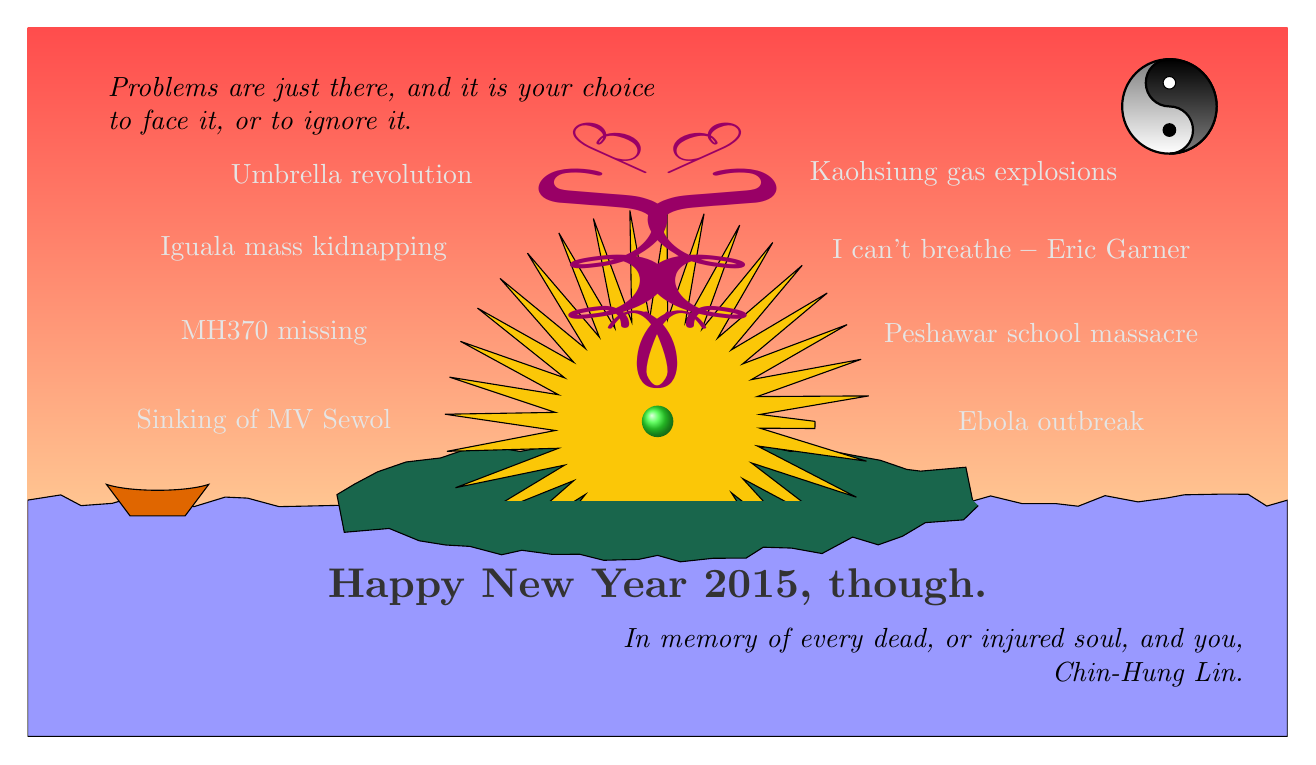
\begin{tikzpicture}
\clip (-8,-4) rectangle (8,5);
%%background Layer
\begin{pgfonlayer}{background}
\shade [top color=red!70, bottom color=yellow!30] (-8,-4) rectangle (8,5);
%\draw [step=1, black, thin] (-8,-4) grid (8,5);
\end{pgfonlayer}

%%main Layer
\begin{pgfonlayer}{main}
%%Tortuga
\draw[fill=blue!40] decorate[decoration={name=random steps}] {(-8,-1) -- (8,-1)} -- (8,-4) -- (-8,-4) -- cycle;
\draw[fill=black!20!red!60!yellow] (-7,-0.8) -- (-6.7,-1.2) -- (-6,-1.2) -- (-5.7,-0.8) .. controls +(-0.3,-0.1) and +(0.3,-0.1) ..  cycle;
\draw[fill=Tortuga] decorate[decoration={name=random steps}] {(0,-1) ellipse [x radius=4cm, y radius=0.7cm]};
\begin{scope}
\clip (-3,-1) rectangle (3,3);
\draw[fill=yellow!80!red] decorate[decoration={name=zigzag,amplitude=0.7cm}] {(0,0) circle [radius=2cm]};
\end{scope}
\node (goatmid) at (0,2.5) {};
\foreach \x in {1.8,-1.8}
{
\begin{scope}[blue!40!red,xscale=\x,scale=1.3,transform shape]
\node[yscale=-1,xshift=-0.75cm,rotate=13,scale=5,right] at (goatmid) {$\xi$};
\node[shift={(-0.4cm,0.4cm)},rotate=65,scale=1.7,right] at (goatmid) {$\beta$};
\node[yscale=-1, yshift=1.2cm,scale=3,rotate=25] at (goatmid) {$\ell$};
\end{scope}
}
\shade[ball color=green!80] (0,0) circle [radius=0.2cm];
%%TaiJi
\begin{scope}[thick,yi/.style={radius=0.4cm},shift={(6.5,4)},scale=0.2]
\shade [draw=black] (0,0) circle [radius =3];
\shade [top color=black, bottom color=black!50,draw=black] (0,-3) arc [radius=3, start angle=-90, end angle=90]
arc [radius=1.5, start angle=90, end angle=270]
arc [radius=1.5, start angle=90, end angle=-90];
\draw[thin,fill=black] (0,-1.5) circle [yi];
\draw[thin,fill=white] (0,1.5) circle [yi];
\end{scope}
\end{pgfonlayer}

%%beta Layer
\begin{pgfonlayer}{beta}
\begin{scope}[black!10]
\foreach \x/\y in {
0/Ebola outbreak,
13/Peshawar school massacre,
26/I can't breathe \textbf{--} Eric Garner,
39/Kaohsiung gas explosions,
180/Sinking of MV Sewol,
167/MH370 missing,
154/Iguala mass kidnapping,
141/Umbrella revolution}
{\node at (\x:5) {\y}; 
}
\end{scope}
\node [black!80,scale=1.5] at (0,-2.1) {\textbf{Happy New Year 2015, though.}};
\node [align=left] at (-3.5,4) {\textit{Problems are just there, and it is your choice }\\\textit{to face it, or to ignore it}.};
\node [align=right] at (3.5,-3) {\textit{In memory of every dead, or injured soul, and you,}\\\textit{Chin-Hung Lin.}};
\end{pgfonlayer}

\end{tikzpicture}
\end{document}
%%\draw=\path[draw]
%%\clip=\path[clip]
%%\graph=\path[graph]
%%bend right ~ bend right=30 ~ in,out=right30, left 30
%%(left:2)=(180:2)
%%left ~ anchor=east ~ anchor 0
%For updating 2.10 to 3.0.0
%after moving the folder, it requires 
%sudo texhash 
% to make it work.
